\documentclass[12pt]{article}
\usepackage[paperwidth=18.5cm, paperheight=16.5cm, margin=0.2cm]{geometry}
\usepackage{tikz}
\usetikzlibrary{positioning, arrows.meta, calc, decorations.pathreplacing}
\pagestyle{empty}
\setlength{\parindent}{0pt}

% ============================================================================
% COLORES Y ESTILOS
% ============================================================================
\definecolor{pastelblue}{RGB}{230, 242, 252}

\tikzset{
  box/.style={
    draw, thick, fill=pastelblue,
    minimum height=1.5cm,
    minimum width=2cm,
    font=\small\sffamily,
    align=center
  },
  ffbox/.style={
    draw, thick, fill=pastelblue,
    minimum width=3.6cm, 
    minimum height=2cm,
    font=\small\sffamily,
    align=center
  },
  signal/.style={-{Stealth[length=2mm]}, thick, black}, 
  wirelabel/.style={font=\tiny\sffamily, text=black, midway, above}
}

% MUX 2-a-1
\newcommand{\drawmux}[4]{
  \draw[thick, fill=pastelblue] (#1-0.4,#2+0.8) -- (#1+0.4,#2+0.4) -- (#1+0.4,#2-0.4) -- (#1-0.4,#2-0.8) -- cycle;
  \node[font=\tiny\sffamily] at (#1-0.15, #2+0.4) {0};
  \node[font=\tiny\sffamily] at (#1-0.15, #2-0.4) {1};
  \coordinate (#3_in0) at (#1-0.4, #2+0.4);
  \coordinate (#3_in1) at (#1-0.4, #2-0.4);
  \coordinate (#3_in2) at (#1-0.4, #2); 
  \coordinate (#3_out) at (#1+0.4, #2);
  \coordinate (#3_sel) at (#1, #2+0.6);
}

% MUX 3-a-1
\newcommand{\drawmuxthree}[4]{
  \draw[thick, fill=pastelblue] (#1-0.4,#2+1.0) -- (#1+0.4,#2+0.6) -- (#1+0.4,#2-0.6) -- (#1-0.4,#2-1.0) -- cycle;
  \node[font=\tiny\sffamily] at (#1-0.15, #2+0.6) {00};
  \node[font=\tiny\sffamily] at (#1-0.15, #2) {01};
  \node[font=\tiny\sffamily] at (#1-0.15, #2-0.6) {10};
  \coordinate (#3_in0) at (#1-0.4, #2+0.6);
  \coordinate (#3_in1) at (#1-0.4, #2);
  \coordinate (#3_in2) at (#1-0.4, #2-0.6);
  \coordinate (#3_out) at (#1+0.4, #2);
  \coordinate (#3_sel) at (#1, #2+0.8);
}

\newcommand{\drawand}[3]{
  \draw[thick, fill=pastelblue] (#1-0.4, #2+0.4) -- (#1, #2+0.4) arc (90:-90:0.4) -- (#1-0.4, #2-0.4) -- cycle;
  \coordinate (#3_in1) at (#1-0.4, #2+0.2);
  \coordinate (#3_in2) at (#1-0.4, #2-0.2);
  \coordinate (#3_out) at (#1+0.4, #2);
}

\newcommand{\drawor}[3]{
  \draw[thick, fill=pastelblue] (#1-0.4, #2+0.4) .. controls (#1-0.1, #2+0.4) and (#1+0.4, #2+0.1) .. (#1+0.4, #2) .. controls (#1+0.4, #2-0.1) and (#1-0.1, #2-0.4) .. (#1-0.4, #2-0.4) .. controls (#1-0.2, #2-0.1) and (#1-0.2, #2+0.1) .. (#1-0.4, #2+0.4) -- cycle;
  \coordinate (#3_in1) at (#1-0.35, #2+0.2);
  \coordinate (#3_in2) at (#1-0.35, #2-0.2);
  \coordinate (#3_out) at (#1+0.4, #2);
}

\newcommand{\drawalu}[3]{
  \draw[thick, fill=pastelblue] 
    (#1-0.8, #2+1.5) -- 
    (#1-0.8, #2+0.3) -- 
    (#1-0.4, #2) -- 
    (#1-0.8, #2-0.3) -- 
    (#1-0.8, #2-1.5) -- 
    (#1+0.8, #2-0.8) -- 
    (#1+0.8, #2+0.8) -- cycle;
  \node[font=\small\sffamily] (#3) at (#1+0.1, #2) {ALU};
  \coordinate (#3_in1) at (#1-0.8, #2+0.8);
  \coordinate (#3_in2) at (#1-0.8, #2-0.8);
  \coordinate (#3_out) at (#1+0.8, #2);
  \coordinate (#3_zero) at (#1+0.8, #2+0.5);
  \coordinate (#3_sel) at (#1, #2+1.1);
}

\newcommand{\drawadder}[3]{
  \draw[thick, fill=pastelblue] 
    (#1-0.6, #2+1.0) -- 
    (#1-0.6, #2+0.2) -- 
    (#1-0.3, #2) -- 
    (#1-0.6, #2-0.2) -- 
    (#1-0.6, #2-1.0) -- 
    (#1+0.6, #2-0.5) -- 
    (#1+0.6, #2+0.5) -- cycle;
  \node[font=\small\sffamily] (#3) at (#1+0.1, #2) {$+$};
  \coordinate (#3_in1) at (#1-0.6, #2+0.5);
  \coordinate (#3_in2) at (#1-0.6, #2-0.5);
  \coordinate (#3_out) at (#1+0.6, #2);
}

\begin{document}
\noindent
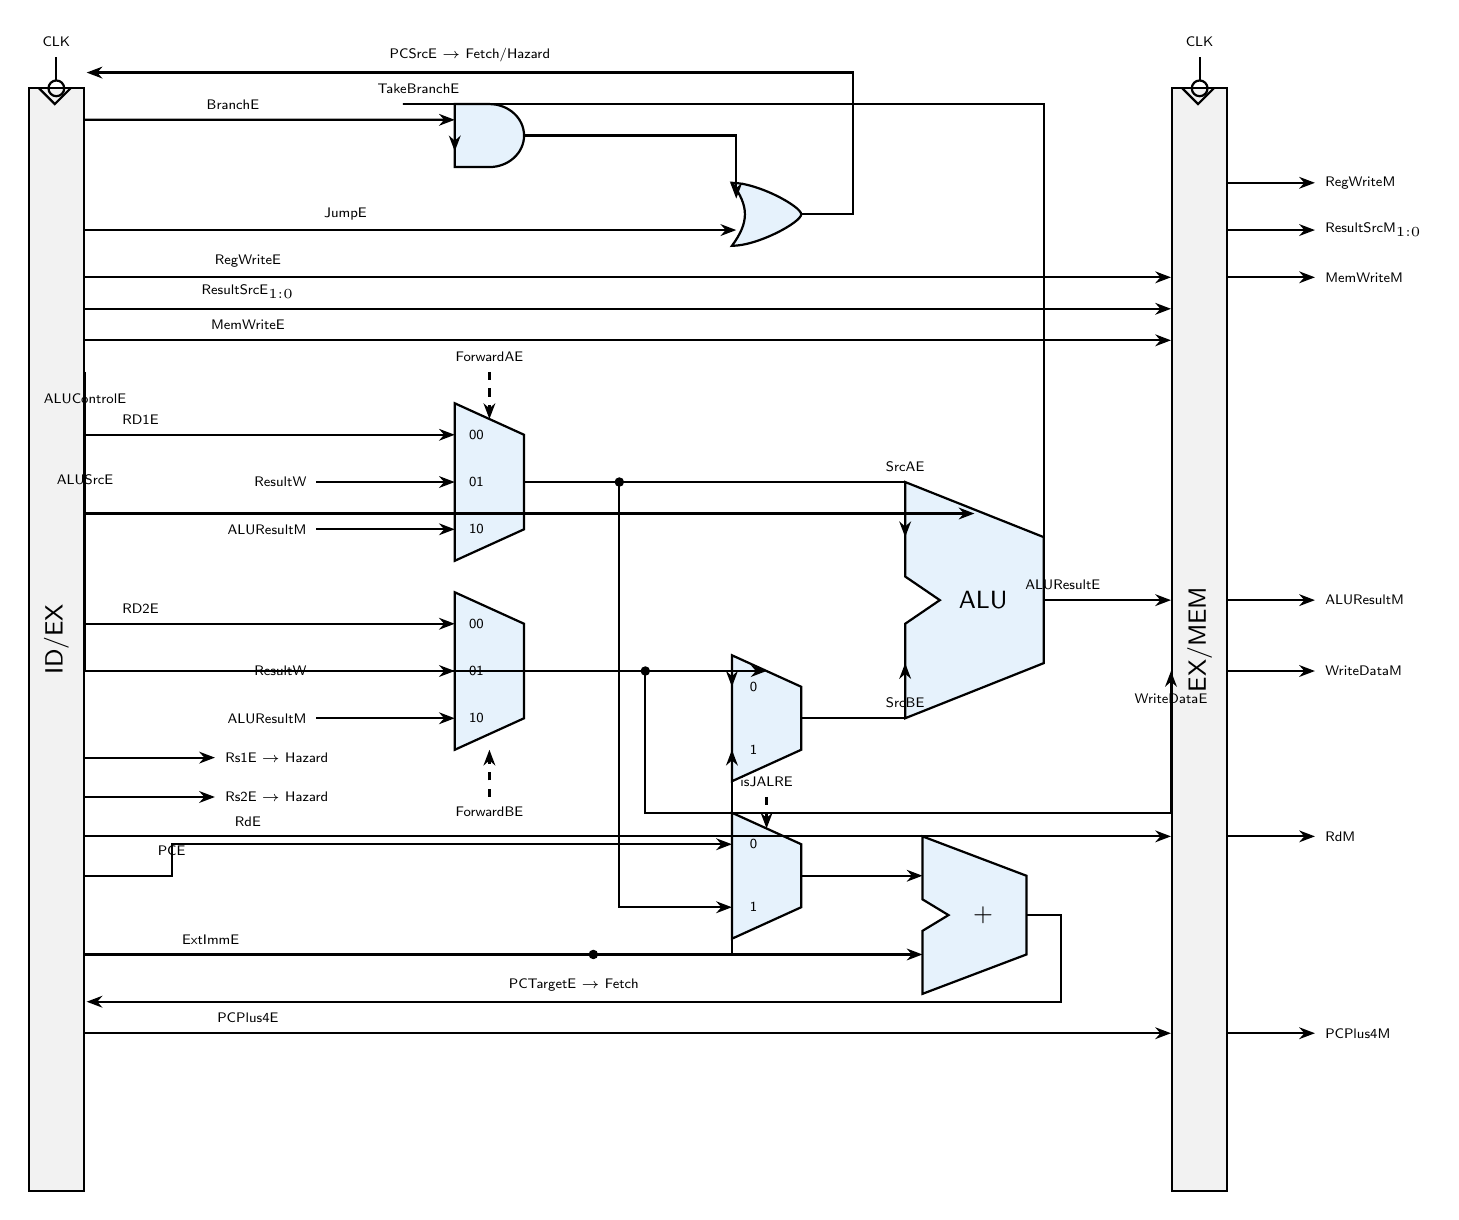
\begin{tikzpicture}[
  x=1.1cm, y=1.0cm,
  signal/.style={-{Stealth[length=2mm]}, thick, black},
  lbl/.style={font=\tiny\sffamily, text=black},
  lblcenter/.style={font=\small\sffamily, align=center},
]

% ID/EX y EX/MEM Pipeline Registers
\node[draw, fill=gray!10, thick, minimum width=0.7cm, minimum height=14cm, font=\small\sffamily] (idex_reg) at (0, 0) {\rotatebox{90}{ID/EX}};
\node[draw, fill=gray!10, thick, minimum width=0.7cm, minimum height=14cm, font=\small\sffamily] (exmem_reg) at (13.2, 0) {\rotatebox{90}{EX/MEM}};

% Clocks
\draw[thick] (0.0, 7.0) circle (1mm);
\draw[thick] (0.0, 7.1) -- ++(0, 3mm) node[above, font=\tiny\sffamily] {CLK};
\draw[thick] (-0.2, 7.0) -- ++(2mm, -2mm) -- ++(2mm, 2mm);

\draw[thick] (13.2, 7.0) circle (1mm);
\draw[thick] (13.2, 7.1) -- ++(0, 3mm) node[above, font=\tiny\sffamily] {CLK};
\draw[thick] (13.0, 7.0) -- ++(2mm, -2mm) -- ++(2mm, 2mm);

% Componentes
\drawmuxthree{5.0}{2.0}{muxA}{}
\drawmuxthree{5.0}{-0.4}{muxB}{}
\drawmux{8.2}{-1.0}{muxS}{}

\drawalu{10.6}{0.5}{myalu}
\drawadder{10.6}{-3.5}{addT}

% Puertas logicas PCSrc
\drawand{5.0}{6.4}{and_gate}
\drawor{8.2}{5.4}{or_gate}

% Control signals top
\draw[signal] (idex_reg.east |- {0, 4.6}) -- (exmem_reg.west |- {0, 4.6}) node[lbl, pos=0.15, above] {RegWriteE};
\draw[signal] (idex_reg.east |- {0, 4.2}) -- (exmem_reg.west |- {0, 4.2}) node[lbl, pos=0.15, above] {ResultSrcE$_{1:0}$};
\draw[signal] (idex_reg.east |- {0, 3.8}) -- (exmem_reg.west |- {0, 3.8}) node[lbl, pos=0.15, above] {MemWriteE};

% Control inputs to MUX and ALU
\draw[signal] (idex_reg.east |- {0, 3.4}) |- (myalu_sel) node[lbl, pos=0.15, above] {ALUControlE};
\draw[signal] (idex_reg.east |- {0, 2.8}) |- (muxS_sel) node[lbl, pos=0.15, above] {ALUSrcE};

% PCSrc Logic Wiring
\draw[signal] (idex_reg.east |- {0, 6.6}) -- (and_gate_in1) node[lbl, pos=0.4, above] {BranchE};
\draw[signal] (idex_reg.east |- {0, 5.2}) -- (or_gate_in2) node[lbl, pos=0.4, above] {JumpE};
\draw[signal] (and_gate_out) -| (or_gate_in1);
\draw[signal] (or_gate_out) -- (9.2, 5.4) |- (9.2, 7.2) -- (0.35, 7.2) node[lbl, midway, above] {PCSrcE $\rightarrow$ Fetch/Hazard};
\draw[signal] (myalu_zero) |- (11.4, 6.8) -- (4.0, 6.8) -| (and_gate_in2) node[lbl, pos=0.15, above] {TakeBranchE};

% RD1E and RD2E inputs to Forwarding Muxes
\draw[signal] (idex_reg.east |- muxA_in0) -- (muxA_in0) node[lbl, pos=0.15, above] {RD1E};
\draw[signal] (idex_reg.east |- muxB_in0) -- (muxB_in0) node[lbl, pos=0.15, above] {RD2E};

% Forwarding inputs represented as clean short lines
\draw[signal] (3.0, 1.4) -- (muxA_in2); \node[left, lbl] at (3.0, 1.4) {ALUResultM};
\draw[signal] (3.0, 2.0) -- (muxA_in1); \node[left, lbl] at (3.0, 2.0) {ResultW};
\draw[signal] (3.0, -1.0) -- (muxB_in2); \node[left, lbl] at (3.0, -1.0) {ALUResultM};
\draw[signal] (3.0, -0.4) -- (muxB_in1); \node[left, lbl] at (3.0, -0.4) {ResultW};

% Selector lines for Forwarding Muxes
\draw[signal, dashed] (5.0, 3.4) node[above, lbl] {ForwardAE} -- (muxA_sel);
\draw[signal, dashed] (5.0, -2.0) node[below, lbl] {ForwardBE} -- (5.0, -1.4);

% MUX outputs -> ALU
\draw[signal] (muxA_out) -| (myalu_in1) node[lbl, midway, above] {SrcAE};
\draw[signal] (muxS_out) -| (myalu_in2) node[lbl, midway, above] {SrcBE};

% WriteDataE
\draw[signal] (muxB_out) -- (6.8, -0.4) |- (6.8, -2.2) -- (12.2, -2.2) -| (exmem_reg.west |- {0, -0.4}) node[lbl, pos=0.85, above] {WriteDataE};
\draw[fill=black] (6.8, -0.4) circle (1.5pt);
\draw[signal] (6.5, -0.4) -- (6.8, -0.4) -| (muxS_in0);

% Mux PC Target Base for JALR
\drawmux{8.2}{-3.0}{jalrmux}{}
\draw[signal] (idex_reg.east |- {0,-3.0}) -- ++(1.0, 0) |- (jalrmux_in0) node[lbl, pos=0.15, above] {PCE};
\draw[fill=black] (6.5, 2.0) circle (1.5pt);
\draw[signal] (6.5, 2.0) |- (jalrmux_in1);
\draw[signal] (jalrmux_out) -- (addT_in1);
\draw[signal, dashed] (8.2, -2.0) node[above, lbl] {isJALRE} -- (jalrmux_sel);

% ExtImmE to Adder and MuxS
\draw[signal] (idex_reg.east |- {0,-4.0}) -- (addT_in2) node[lbl, pos=0.15, above] {ExtImmE};
\draw[fill=black] (6.2, -4.0) circle (1.5pt);
\draw[signal] (6.2, -4.0) -| (muxS_in1);

% Pass-through signals to Hazard Unit or next stage
\draw[signal] (idex_reg.east |- {0, -1.5}) -- ++(1.5, 0) node[right, lbl] {Rs1E $\rightarrow$ Hazard};
\draw[signal] (idex_reg.east |- {0, -2.0}) -- ++(1.5, 0) node[right, lbl] {Rs2E $\rightarrow$ Hazard};
\draw[signal] (idex_reg.east |- {0, -2.5}) -- (exmem_reg.west |- {0,-2.5}) node[lbl, pos=0.15, above] {RdE};
\draw[signal] (idex_reg.east |- {0, -5.0}) -- (exmem_reg.west |- {0,-5.0}) node[lbl, pos=0.15, above] {PCPlus4E};

% Outputs from EX passing right
\draw[signal] (myalu_out) -- (exmem_reg.west |- myalu_out) node[lbl, pos=0.15, above] {ALUResultE};
\draw[signal] (addT_out) -- (11.6, -3.5) |- (11.6, -4.6) -- (0.35, -4.6) node[lbl, midway, above] {PCTargetE $\rightarrow$ Fetch};

% Labeled outputs on the east of EX/MEM register
\draw[signal] (exmem_reg.east |- myalu_out) -- ++(1.0, 0) node[right, lbl] {ALUResultM};
\draw[signal] (exmem_reg.east |- {0, -0.4}) -- ++(1.0, 0) node[right, lbl] {WriteDataM};
\draw[signal] (exmem_reg.east |- {0,-2.5}) -- ++(1.0, 0) node[right, lbl] {RdM};
\draw[signal] (exmem_reg.east |- {0,-5.0}) -- ++(1.0, 0) node[right, lbl] {PCPlus4M};
\draw[signal] (exmem_reg.east |- {0,5.8}) -- ++(1.0, 0) node[right, lbl] {RegWriteM};
\draw[signal] (exmem_reg.east |- {0,5.2}) -- ++(1.0, 0) node[right, lbl] {ResultSrcM$_{1:0}$};
\draw[signal] (exmem_reg.east |- {0,4.6}) -- ++(1.0, 0) node[right, lbl] {MemWriteM};

\end{tikzpicture}
\end{document}
